\appendix
\newpage
\part*{\Huge Appendix}

% \section{Possible Questions}

% \chen{do we really want to include this section?}
% \paragraph{Q:}\textit{What is the Difference between PDM-Pure and Diff-Pure~\cite{nie2022diffusion}?}

% Diff-Pure~\cite{nie2022diffusion} is proposed to purify 

% \paragraph{Q:}\textit{Can Adaptive Attacks be Used to Attack PDM-Pure?}

% Since PDM-Pure can be used to purify protective perturbations, can we develop stronger adaptive attacks targeting the purification process? Actually, ~\cite{zhao2023can} already did experiments to adaptively attack DiffPure and the answer is that the protection still does not work. It further reflects our conclusion that PDM is robust.




\section{Details about Different Diffusion Models in this Paper}

Here we introduce the diffusion models used in this work, which cover different types of diffusion (LDM, PDM), different training datasets, different resolutions, and different model structures (U-Net, Transformer):

\paragraph{Guided Diffusion (PDM)} We use the implementation and checkpoint from \url{https://github.com/openai/guided-diffusion}, the Guided Diffusion models we used are trained on ImageNet~\cite{deng2009imagenet} in resolution $256\times 256$, the editing results are tested on sub-dataset of ImageNet validation set sized 500.

\paragraph{IF-Stage I (PDM)} This is the first stage of the cascaded DeepFloyd IF model~\cite{deepfloyd} from \url{https://github.com/deep-floyd/IF}. It is trained on LAION 1.2B with text annotation. It has a resolution of $64\times 64$. the editing results are tested on the image dataset introduced in ~\cite{sdsattack}, including 400 anime, portrait, landscape, and artwork images.

\paragraph{IF-Stage II (PDM)} This is the second stage of the cascaded DeepFloyd IF model~\cite{deepfloyd} from \url{https://github.com/deep-floyd/IF}. It is a conditional diffusion model in the pixel space with $256\times 256$, which is conditioned on $64\times 64$ low-resolution images. During the attack, we freeze the image condition and only attack the target image to be edited.

% \chen{how about IF-Stage III?}\haotian{stage iii is for super-resolution in 1024*1024, the pixel-space version is not opensource, the opensource one uses SD}

\paragraph{Stable Diffusion V-1.4 (LDM)}
It is one of the most popular LDMs from \url{https://huggingface.co/CompVis/stable-diffusion-v1-4}, also trained on text-image pairs, which has been widely studied in this field. It supports resolutions of $256\times 256$ and $512\times 512$, both can be easily attacked. The encoder first encodes the image sized $H\times W$ into the latent space sized $4\times H/4 \times W/4$, and then uses U-Net combined with cross-attention to run the denoising process.

\paragraph{Stable Diffusion V-1.5 (LDM)}
It has the same structure as Stable Diffusion V-1.4, which is also stronger since it is trained with more steps, from \url{https://huggingface.co/runwayml/stable-diffusion-v1-5}.

\paragraph{DiT-XL (LDM)} It is another popular latent diffusion model, that uses the backbone of the Transformer instead of the U-Net. We use the implementation from the original repository \url{https://github.com/facebookresearch/DiT/}. 



\section{Details about Different Protection Methods in this Paper}
We introduce different protection methods tested in this paper, of which all the original versions are designed for LDMs. All the adversarial attacks work under the white box settings of PGD-attack, varying from each other with different adversarial losses:


\paragraph{AdvDM} AdvDM is one of the first adversarial attacks proposed in ~\cite{advdm}, it used a Monte-Carlo-based adversarial loss which can effectively attack the latent diffusion models, we also call this loss semantic loss:

\begin{equation}\label{appendix:semantic_loss}
        \mathcal{L}_{S}(x) = \mathbb{E}_{t, \epsilon} \mathbb{E}_{z_t \sim q_t(\mathcal{E}_{\phi}(x))}\|\epsilon_{\theta}(z_t, t) -\epsilon \|_2^2
\end{equation}


\paragraph{PhotoGuard} PhotoGuard is proposed in ~\cite{salman2023raising}, it takes the encoder, making the encoded image close to a target image $y$, we also call it textural loss:

\begin{equation}\label{appendix:tex-loss}
        \mathcal{L}_{T}(x) = -\|\mathcal{E}_{\phi}(x) -\mathcal{E}_{\phi}(y) \|_2^2
    \end{equation}

\paragraph{Mist} Mist~\cite{liang2023mist} finds that ${L}_{T}(x)$ can better enhance the attacks if the target image $y$ is chosen to be periodical patterns, the final loss combined ${L}_{T}(x)$ and ${L}_{S}(x)$:

\begin{equation}
    \mathcal{L} = \lambda {L}_{T}(x) + {L}_{S}(x)
\end{equation}

\paragraph{SDS(+)} Proposed in ~\cite{sdsattack}, it is proven to be a more effective attack compared with the original AdvDM, where the gradient $\nabla_x\mathcal{L}(x)$ is expensive to compute. By using the score distillation-based loss, it shows good performance and remains effective at the same time:

\begin{equation}\label{sds_equation}
    \nabla_{x}\mathcal{L}_{SDS}(x) =  \mathbb{E}_{t, \epsilon}\mathbb{E}_{z_t} \left[\lambda(t) (\epsilon_{\theta}(z_t, t) -\epsilon)\frac{\partial z_t}{\partial x_t}\right]
\end{equation}

\paragraph{SDS(-)} Similar to SDS(+), it swaps gradient ascent in the original PGD with gradient descent, which turns out to be even more effective.

\begin{equation}\label{sds_equation}
    \nabla_{x}\mathcal{L}_{SDS(-)}(x) = -\mathbb{E}_{t, \epsilon}\mathbb{E}_{z_t} \left[\lambda(t) (\epsilon_{\theta}(z_t, t) -\epsilon)\frac{\partial z_t}{\partial x_t}\right]
\end{equation}



\paragraph{Mist-v2} It was proposed in ~\cite{mist-v2} using the Improved Targeted Attack (ITA), which turns out to be very effective, especially when the limit budget is small. It is also more effective to attack LoRA:

\begin{equation}
     \mathcal{L}_{S}(x) = \mathbb{E}_{t, \epsilon} \mathbb{E}_{z_t \sim q_t(\mathcal{E}_{\phi}(x))}\|\epsilon_{\theta}(z_t, t) -z_0 \|_2^2
\end{equation}

where $z_0 = \mathcal{E}(y)$ is the latent of a target image, which is the same as the typical image used in Mist.

\paragraph{Glaze} It is the most popular protection claimed to safeguard artists from unauthorized imitation~
\cite{glaze} and is widely used by the community. while it is not open-sourced, it also attacks the encoder like the Photoguard. Here we only test it in the purification stage, where we show that the protection can also be bypassed.

% \paragraph{MetaCloak} It is proposed in~\cite{metacloak} which is strong against different kinds of purification, we also test it in the PDM-Pure stage.

\paragraph{End-to-End Attack} It is also first proposed in ~\cite{salman2023raising}, which attacks the editing pipeline in a end-to-end manner. Although it is strong, it is not practical to use and does not show dominant privilege compared with other protection methods.

\section{Details about The Evaluation Metrics}\label{supp:section:eval_metrics}

 Here we introduce the quantitative measurement we used in our experiments: 

 \begin{itemize}
     \item We measure the SDEdit results after the adversarial attacks using Fréchet Inception Distance (FID)~\citep{fid} over the relevant datasets (for model trained on ImageNet such as GD~\cite{guideddiffusion} and DiT~\cite{dit} we use a sub-dataset of ImageNet as the relevant dataset, for those trained on LAION, we use the collected dataset to calculate the FID). We also use Image-Alignment Score (IA-score)~\citep{la-score}, which can be used to calculate the cosine-similarity between the CLIP embedding of the edited image and the original image. Also, we use some basic evaluations, where we calculate the Structural Similarity (SSIM)~\citep{ssim} and Perceptual Similarity (LPIPS)~\citep{lpips} compared with the original images.

     \item To measure the purification results, we test the Fréchet Inception Distance (FID)~\citep{fid} over the collected dataset compared with the dataset generated by running SDEdit over the purified images in the strength of $0.3$.
 \end{itemize}
 
 % (2) To measure the protection results, we use FID, LPIPS, Peak Signal-to-Noise Ratio (PSNR)~\citep{psnr}, and Image-Alignment Score (IA-score)~\citep{la-score} which calculated the cosine-similarity between the CLIP embedding of the protected image and the original image. Also, we have human evaluations which are collected using surveys, which is a more convincing way to evaluate the quality of protections, more settings can be found in the appendix.





\section{Details about Different Purification Methods}\label{supp:section:purification_baselines}


\paragraph{Adv-Clean:} \url{https://github.com/lllyasviel/AdverseCleaner}, a training-free filter-based method that can remove adversarial noise for a diffusion model, it works well to remove high-frequency noise.

\paragraph{Crop $\&$ Resize:} we first crop the image by $20\%$ and then resize the image to the original size, it turns out to be one of the most effective defense methods \citep{liang2023mist}.

\paragraph{JPEG compression:} \citep{sandoval2023jpeg} reveals that JPEG compression can be a good purification method, and we adopt the $65\%$ as the quality of compression in \citep{sandoval2023jpeg}.

\paragraph{LDM-Pure:} We also try to use LDMs to run SDEdit as a naive purifier, sadly it cannot work, because the adversarial protection transfers well between different LDMs.

\paragraph{GrIDPure:} It is proposed in ~\cite{zhao2023can} as a purifier, GrIDPure first divides an image into patches sized $128\times 128$, and then purifies the $9$ patches sized $256\times 256$. Also, it combined the four corners sized $128\times 128$ to purify it so we have $10$ patches to purify in total. After running SDEdit with a small noise (set to $0.1 T$), we reassemble the patches into the original size, pixel values are assigned using the average values of the patches they belong to. More details can be seen in ~\cite{zhao2023can}.


\section{More Experimental Results}

In this section, we present more experimental results.

\subsection{More Visualizations of Attacking PDMs}

We show more results of attacking LDMs and PDMs in Figure~\ref{fig:supp:attacking_pdms}, where we attack them with different budget $\delta=4,8,16$. We can see all the LDMs can be easily attacked, while PDMs cannot be attacked, even the largest perturbations will not fool the editing process. Actually, the editing process is trying to purify the strange perturbations.

\begin{figure}
    \centering
    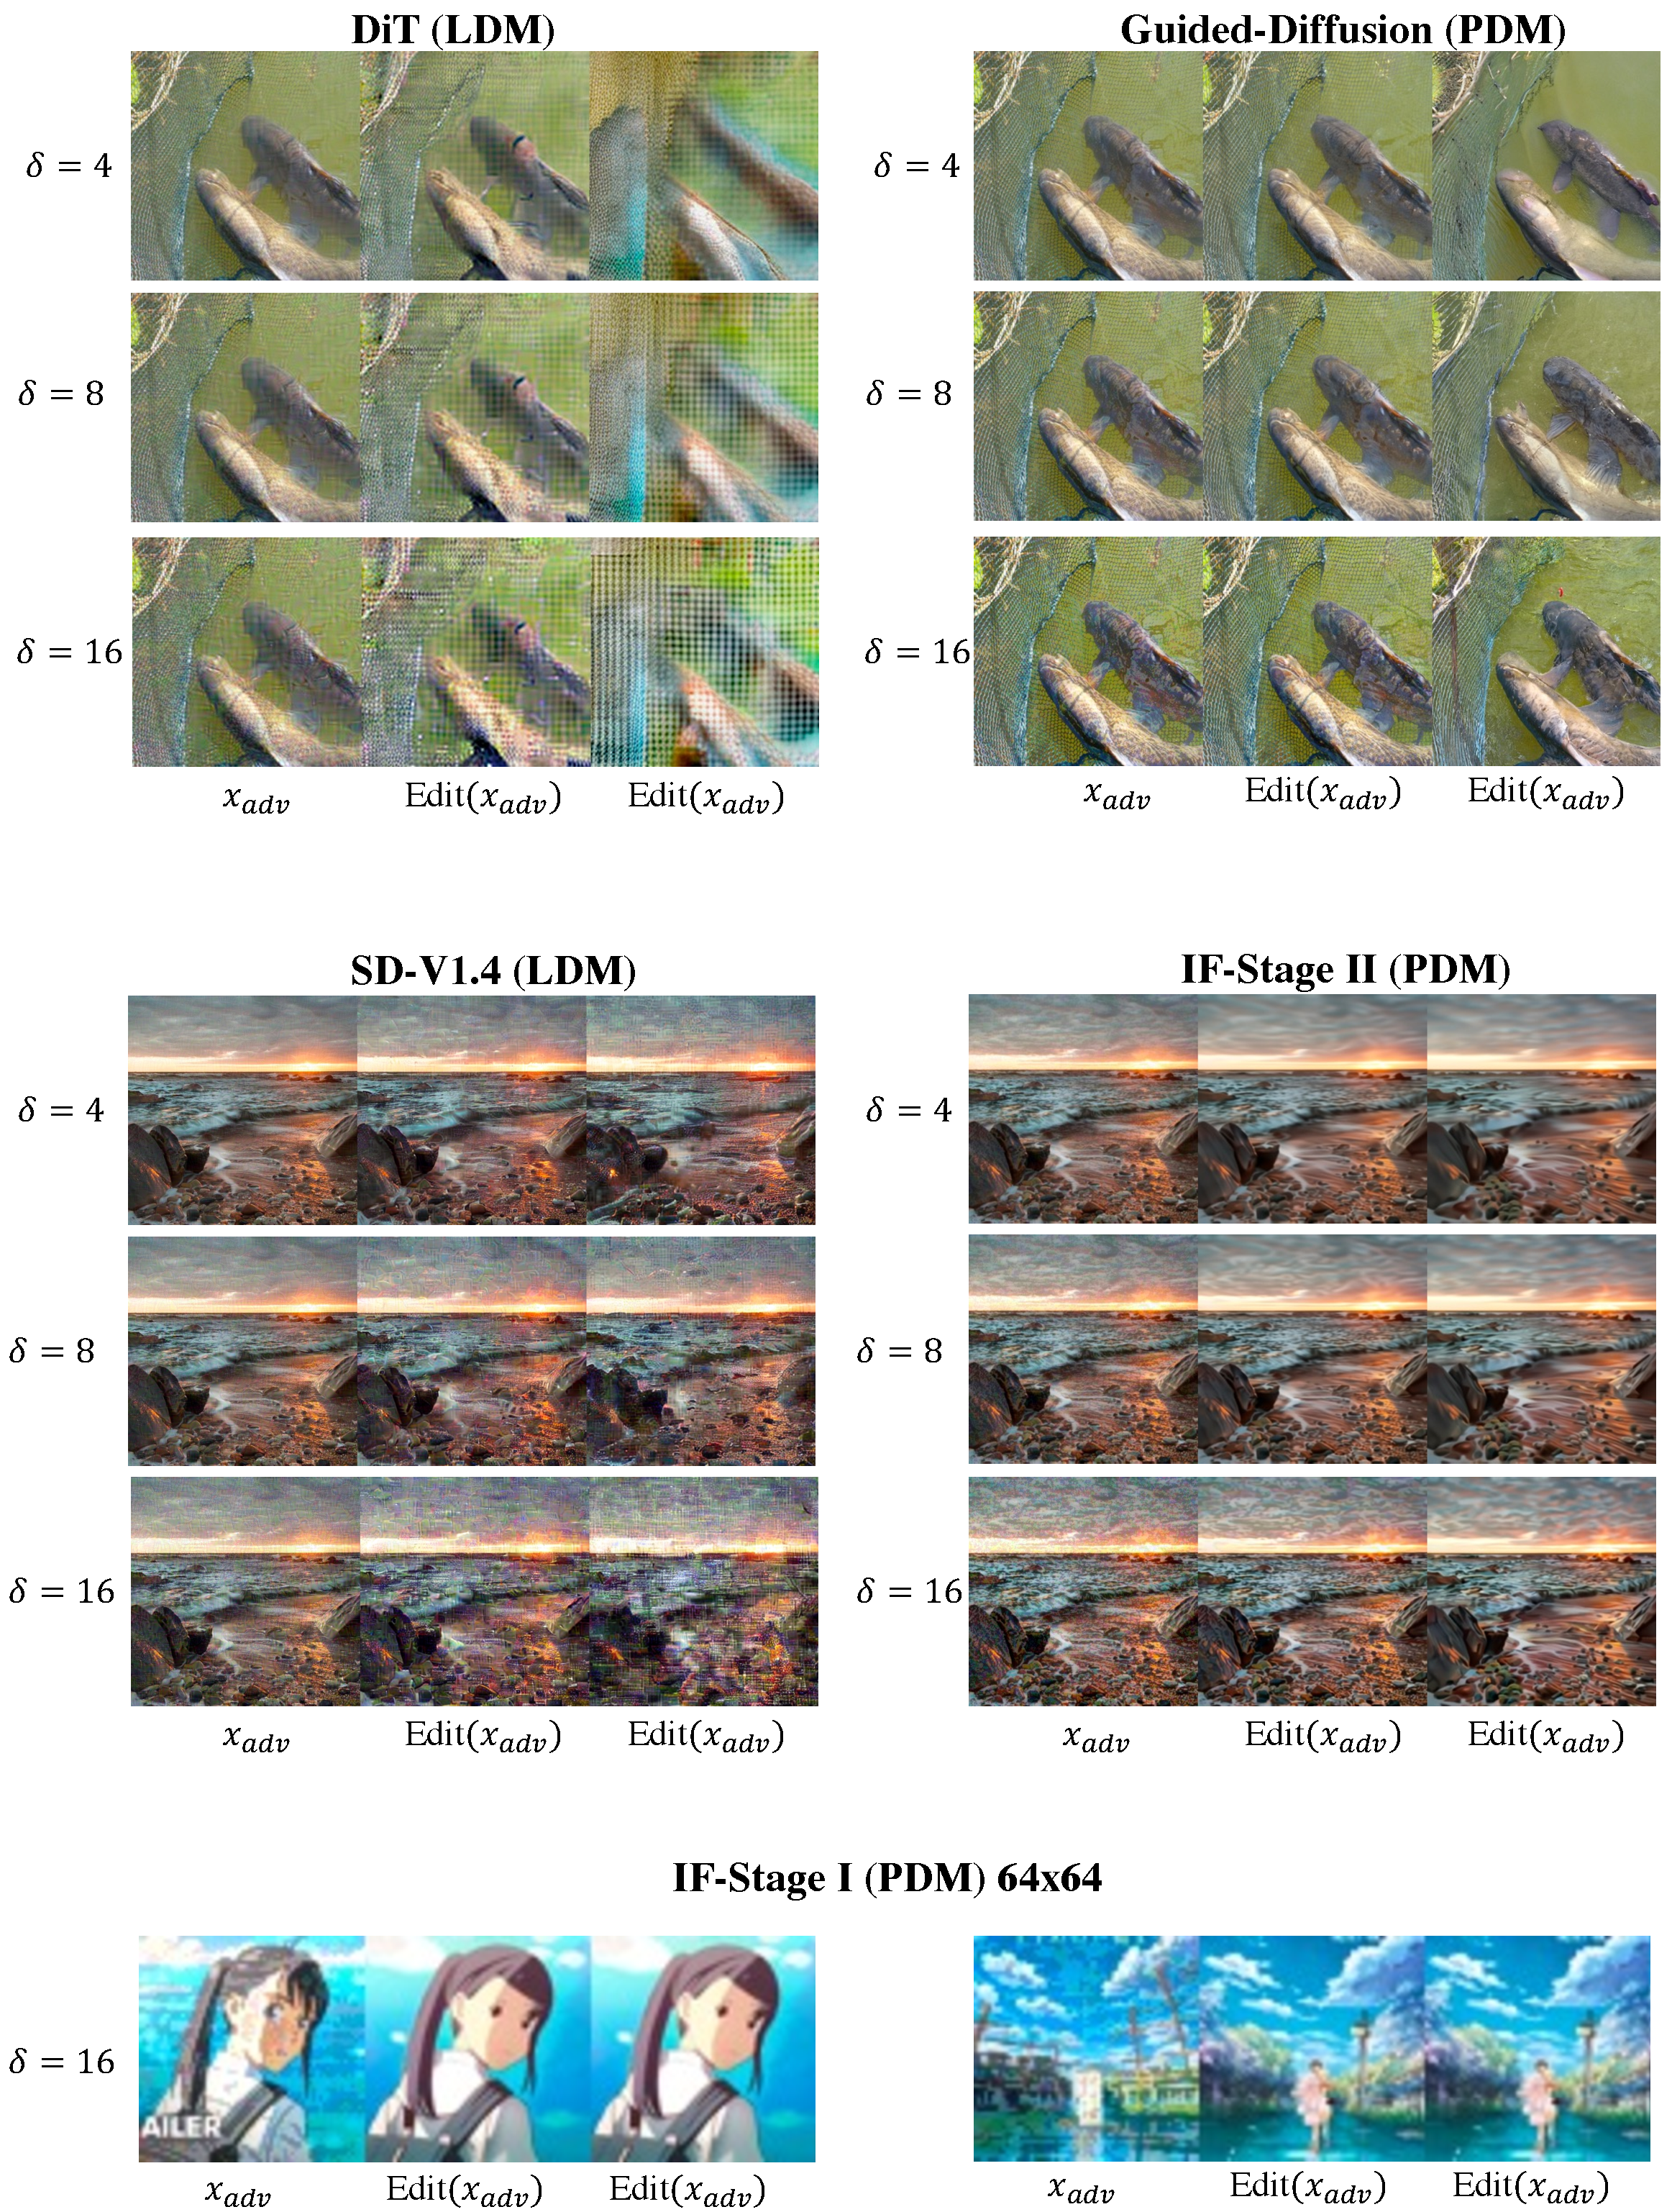
\includegraphics[width=.99\textwidth]{images/supp/supp_attacking_pdms.pdf}
    \caption{\textbf{PDMs cannot be Attacked as LDMs}: we conduct experiments on various models with various budgets, even the largest budget will not affect the PDMs, showing that PDMs are adversarially robust. For each block, the first column is the attacked image, and the second and third columns are edited images, where the third column adopts larger editing strength.}
    \label{fig:supp:attacking_pdms}
\end{figure}






\subsection{More Visualizaitons of PDM-Pure and Baseline Methods}

We show more qualitative results of the proposed PDM-Pure based on IF. First, we show purified samples of PDM-Pure in Figure.~\ref{fig:supp:pdm_pure_visualize}, from which we can see that PDM-Pure can remove large protective perturbations and largely preserve details. 

Compared with GrIDPure~\cite{zhao2023can}, we find that PDM-Pure shows better results when the noise is large and colorful, as is illustrated in Figure~\ref{fig:supp:pdm_pure_compared with gridpure}. Also, though GrIDPure merges patches, it still shows boundary lines between patches. 

Compared with other baseline purification methods such as Adv-Clean, Crop-and-Resize, and JPEG compression, PDM-Pure shows much better results (Figure~\ref{fig:supp:different_purification_methods}) for different kinds of protective noise, showing that it is capable to serve as a universal purifier. We choose AdvDM, Mist, and SDS as the representative of three kinds of protection. 

\begin{figure}
    \centering
    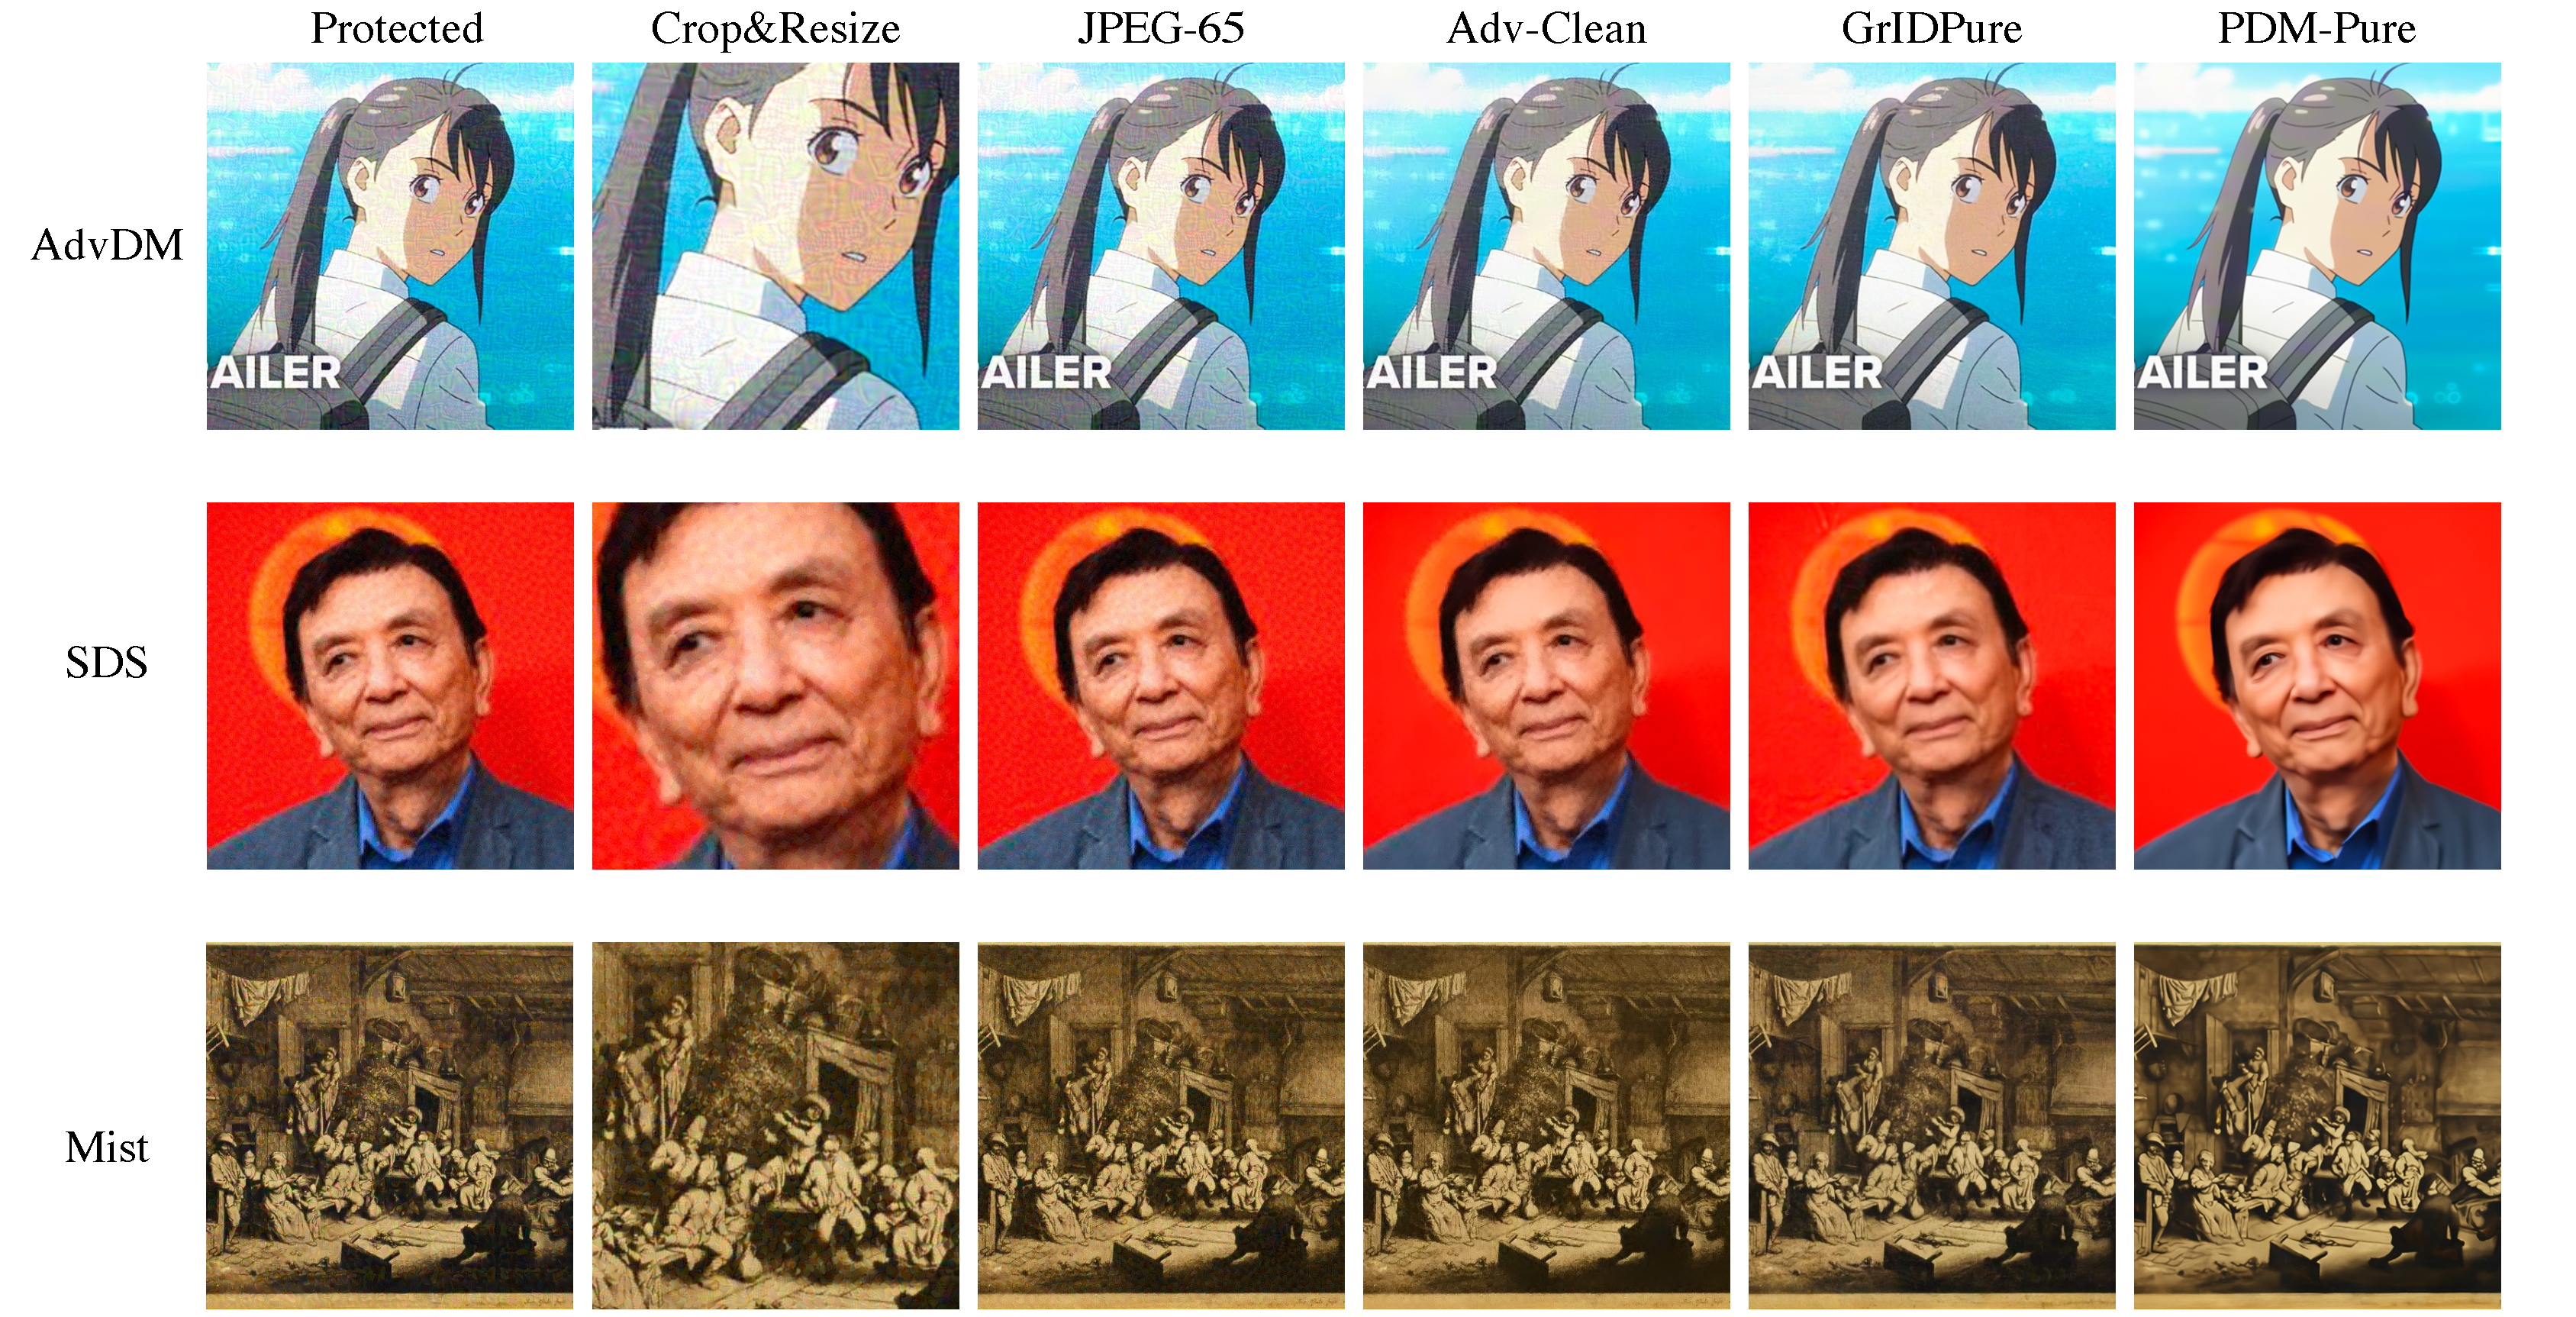
\includegraphics[width=.99\textwidth]{images/supp/different_purification_methods.pdf}
    \caption{
    % \chen{all the methods seem to be effective}\haotian{baselines still show adversarial patterns}
    \textbf{PDM-Pure Compared With Other Baseline Methods}: we test all the baselines on three typical kinds of protection methods, with $\delta=16/255$. PDM-Pure shows strong performance.}
    \label{fig:supp:different_purification_methods}
\end{figure}


\begin{figure}
    \centering
    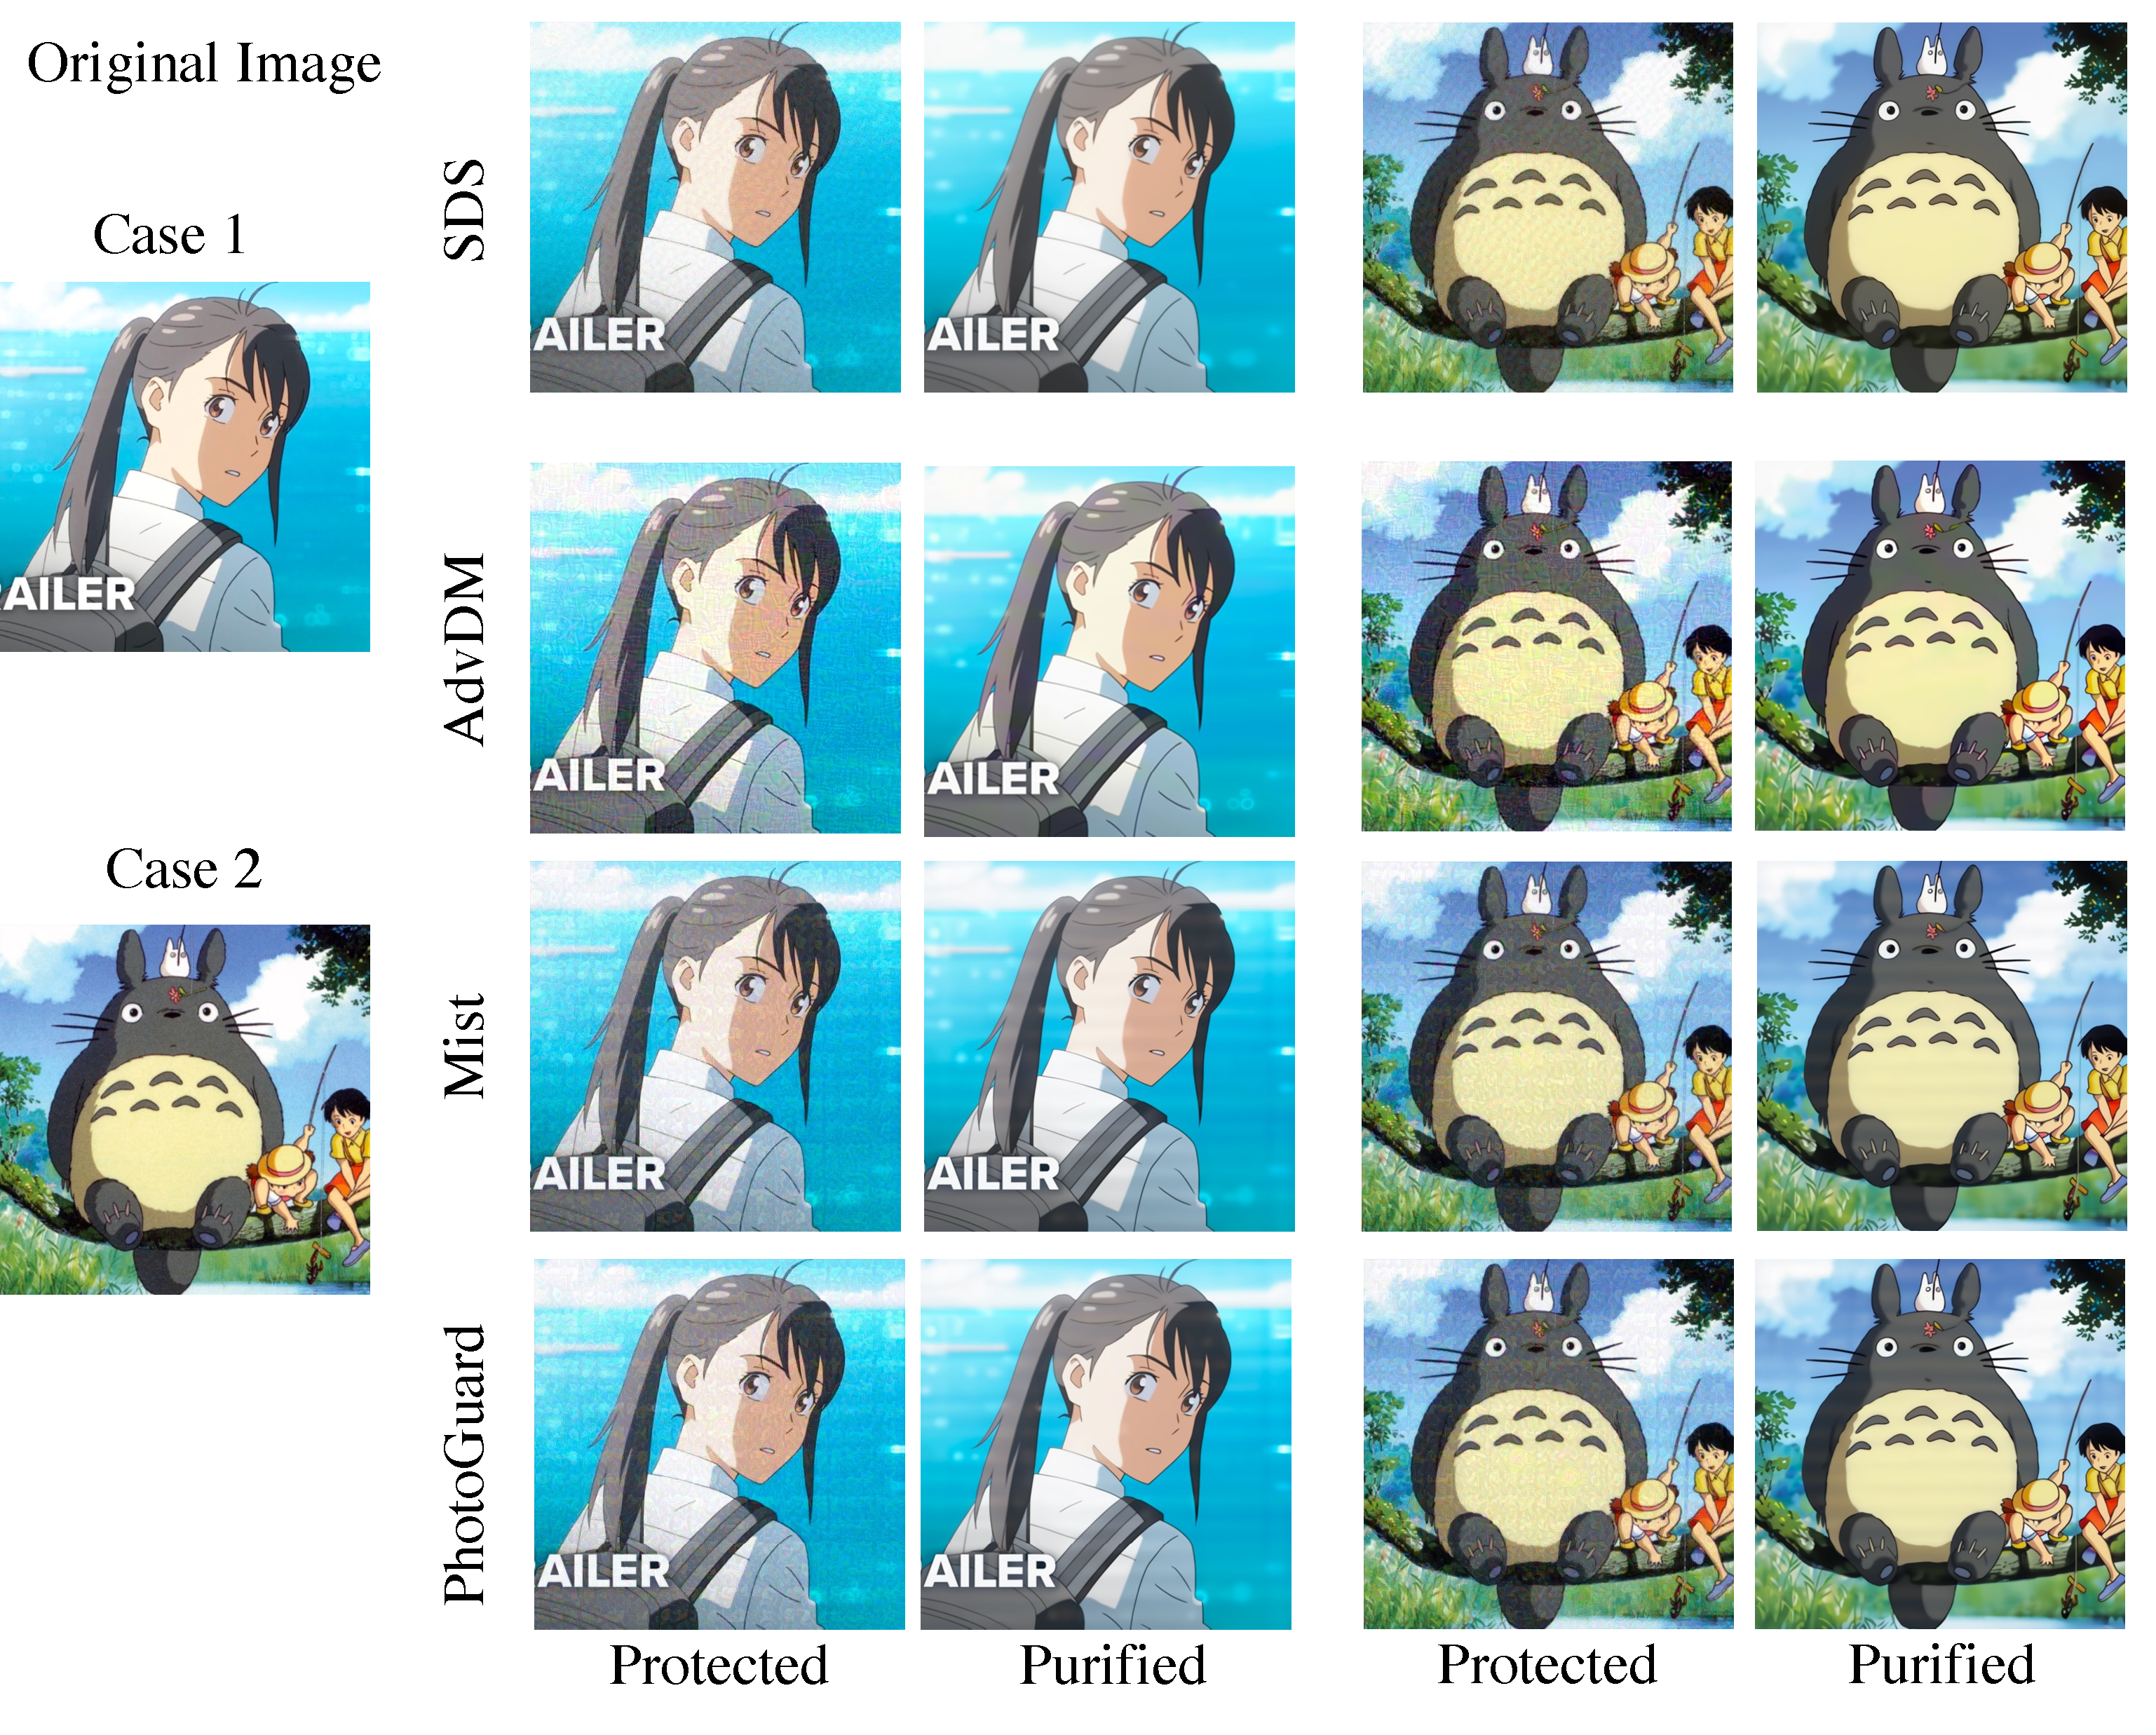
\includegraphics[width=.99\textwidth]{images/supp/pdm_pure_visualize.pdf}
    \caption{\textbf{More Purification Results of PDM-Pure}: we show purification results compared with the clean image, working on SDS, AdvDM, Mist, and PhotoGuard.}
    \label{fig:supp:pdm_pure_visualize}
\end{figure}

\begin{figure}
    \centering
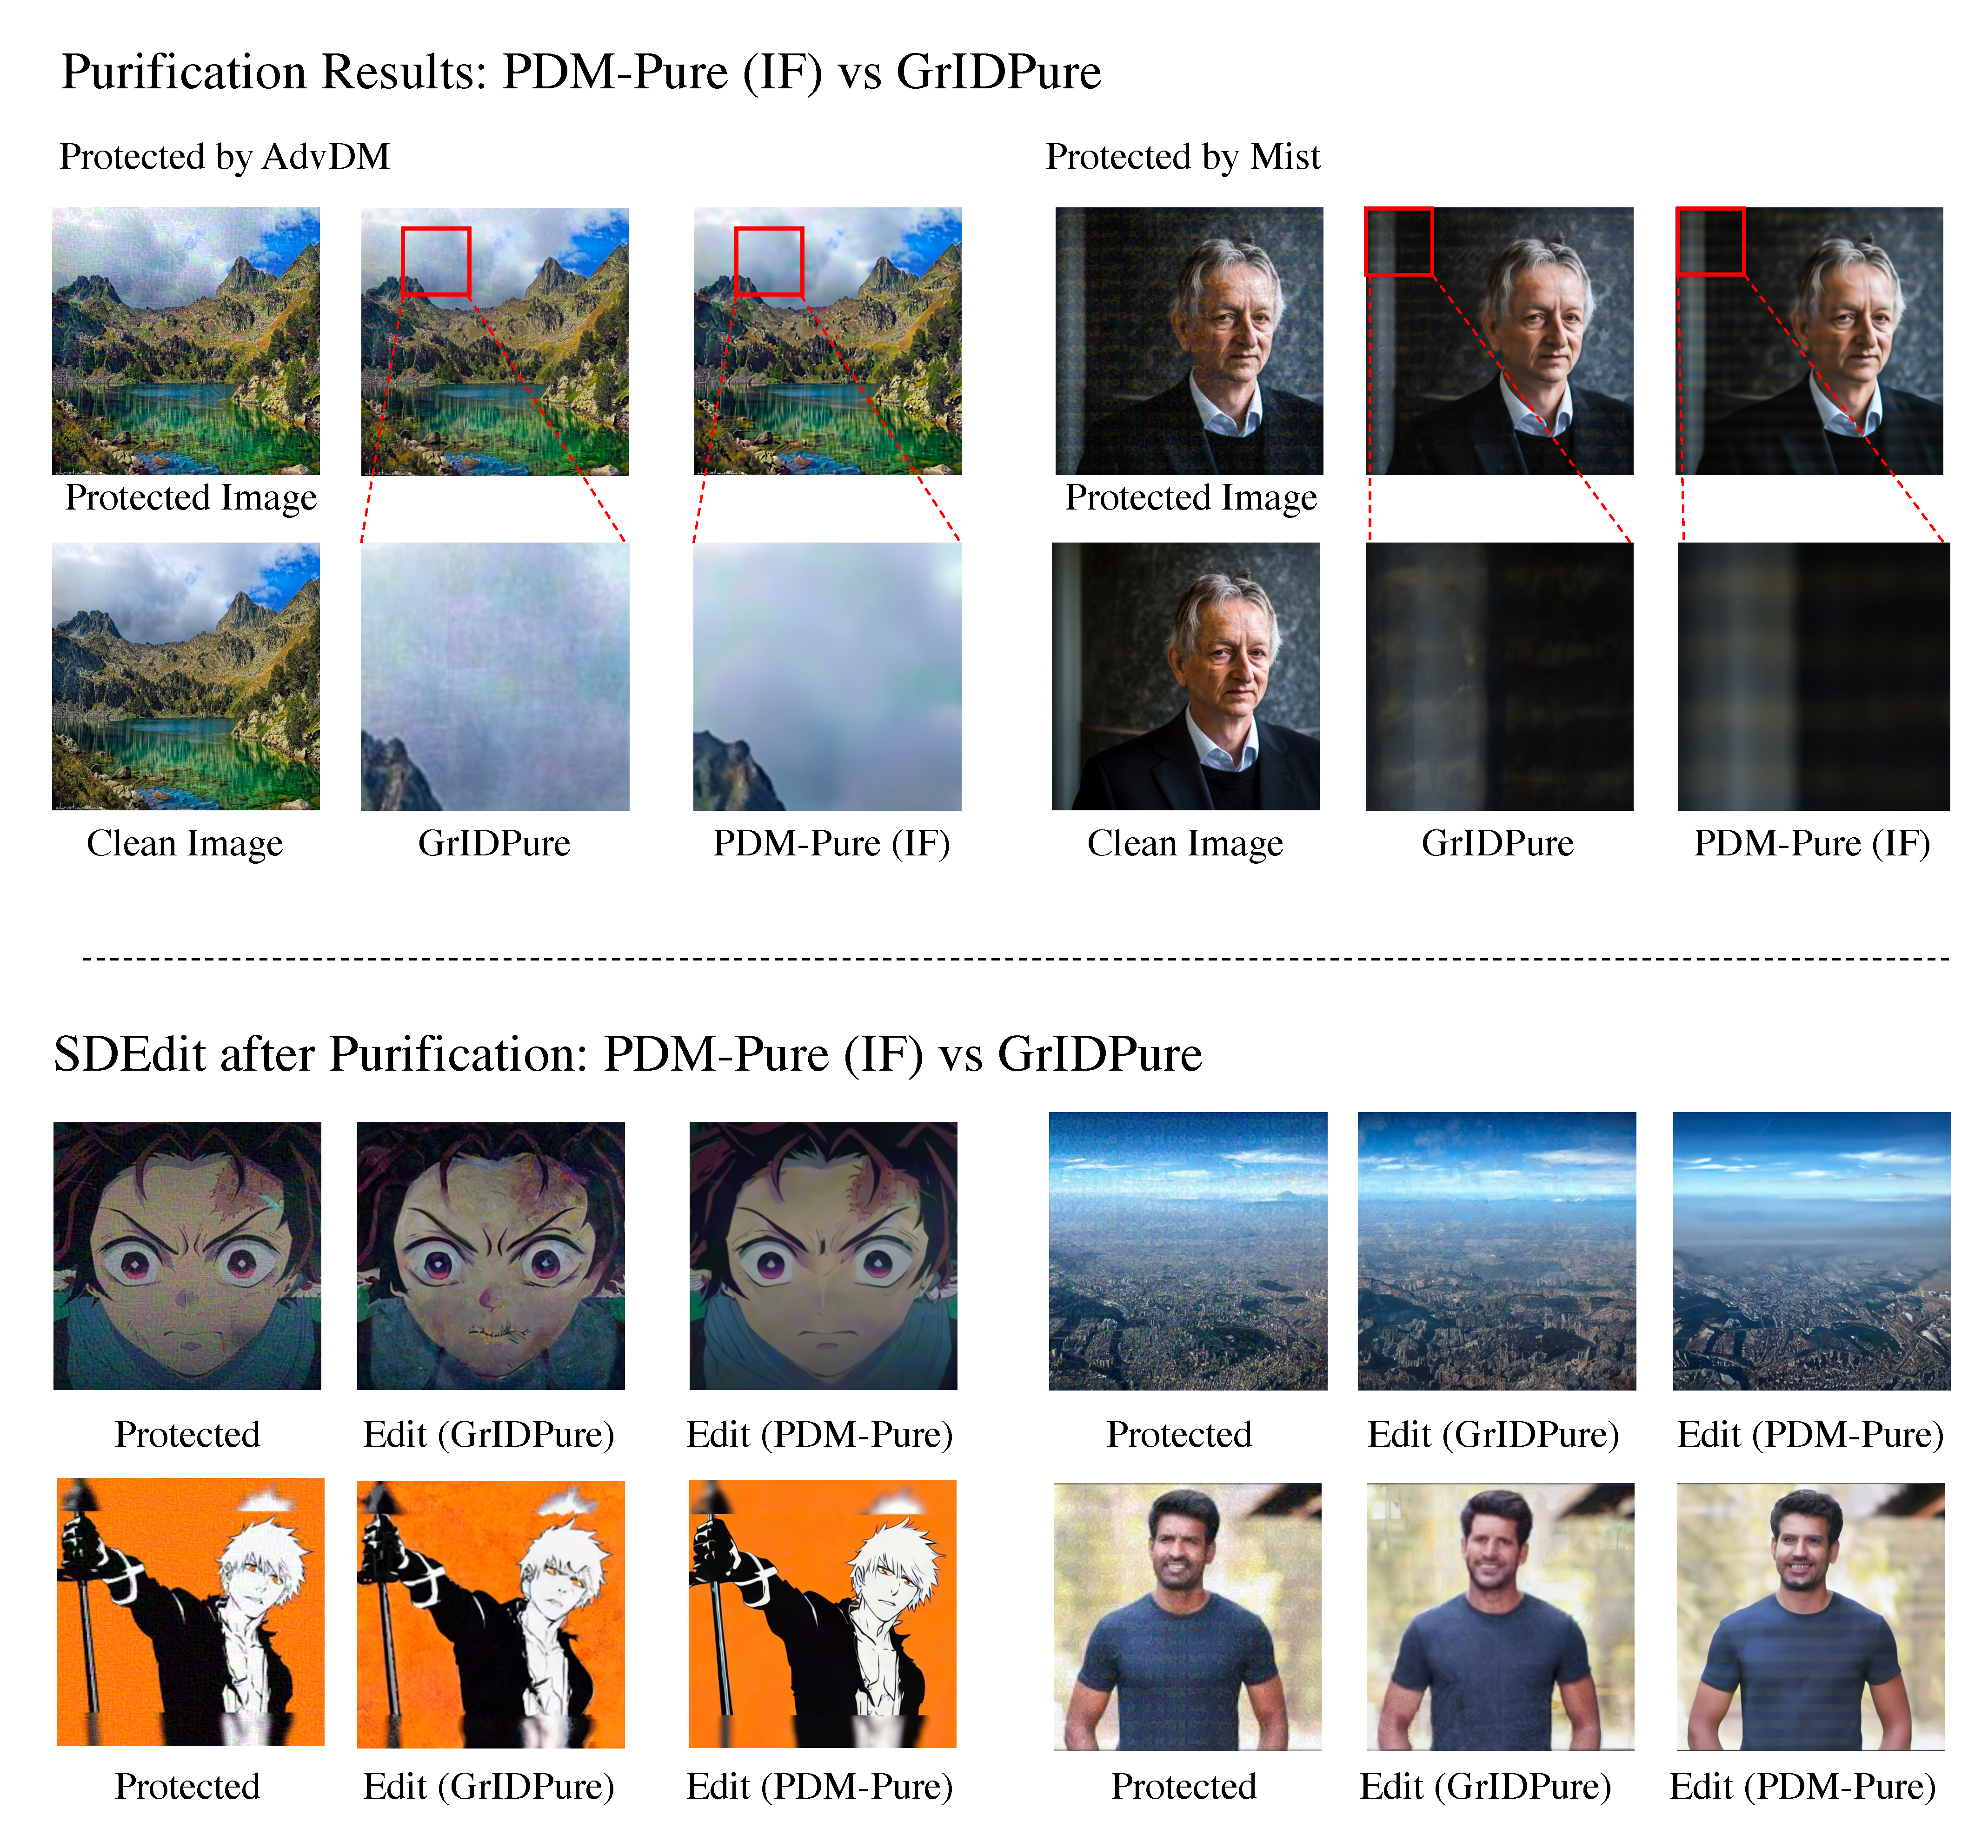
\includegraphics[width=.99\textwidth]{images/supp/pdm_pure_baselines.pdf}
    \caption{
    % \chen{why is the protected one so good?}\haotian{oh, it is not editing results, it is just the original image} 
    \textbf{PDM-Pure vs GrIDPure}: PDM-Pure is better than GrIDPure, especially when the adversarial pattern is strong such as AdvDM. The bottom half of this figure shows the editing results of purified images, we can see that the editing results of GrIDPure still show somewhat artifacts.}
    \label{fig:supp:pdm_pure_compared with gridpure}
\end{figure}


\subsection{More Visualizaitons of PDM-Pure for Downstreaming Tasks}

After applying PDM-Pure to the protected images, they are no longer adversarial to LDMs and can be easily edited or imitated. Here we will demonstrate more results on editing the purified images on downstream tasks.


In Figure~\ref{fig:supp:pdm_pure_inpainting}, we show more results to prove that the purified images can be edited easily, and the quality of editing results is high. It means that PDM-Pure can bypass the protection very well for inpainting tasks.

In Figure~\ref{fig:supp:pdm_pure_lora} we show more results on purifying Mist~\cite{liang2023mist} and Glaze~\cite{glaze} perturbations, and then running LoRA customized generation. From the figure, we can see that PDM-Pure can make the protected images easy to imitate again.

\begin{figure}
    \centering
    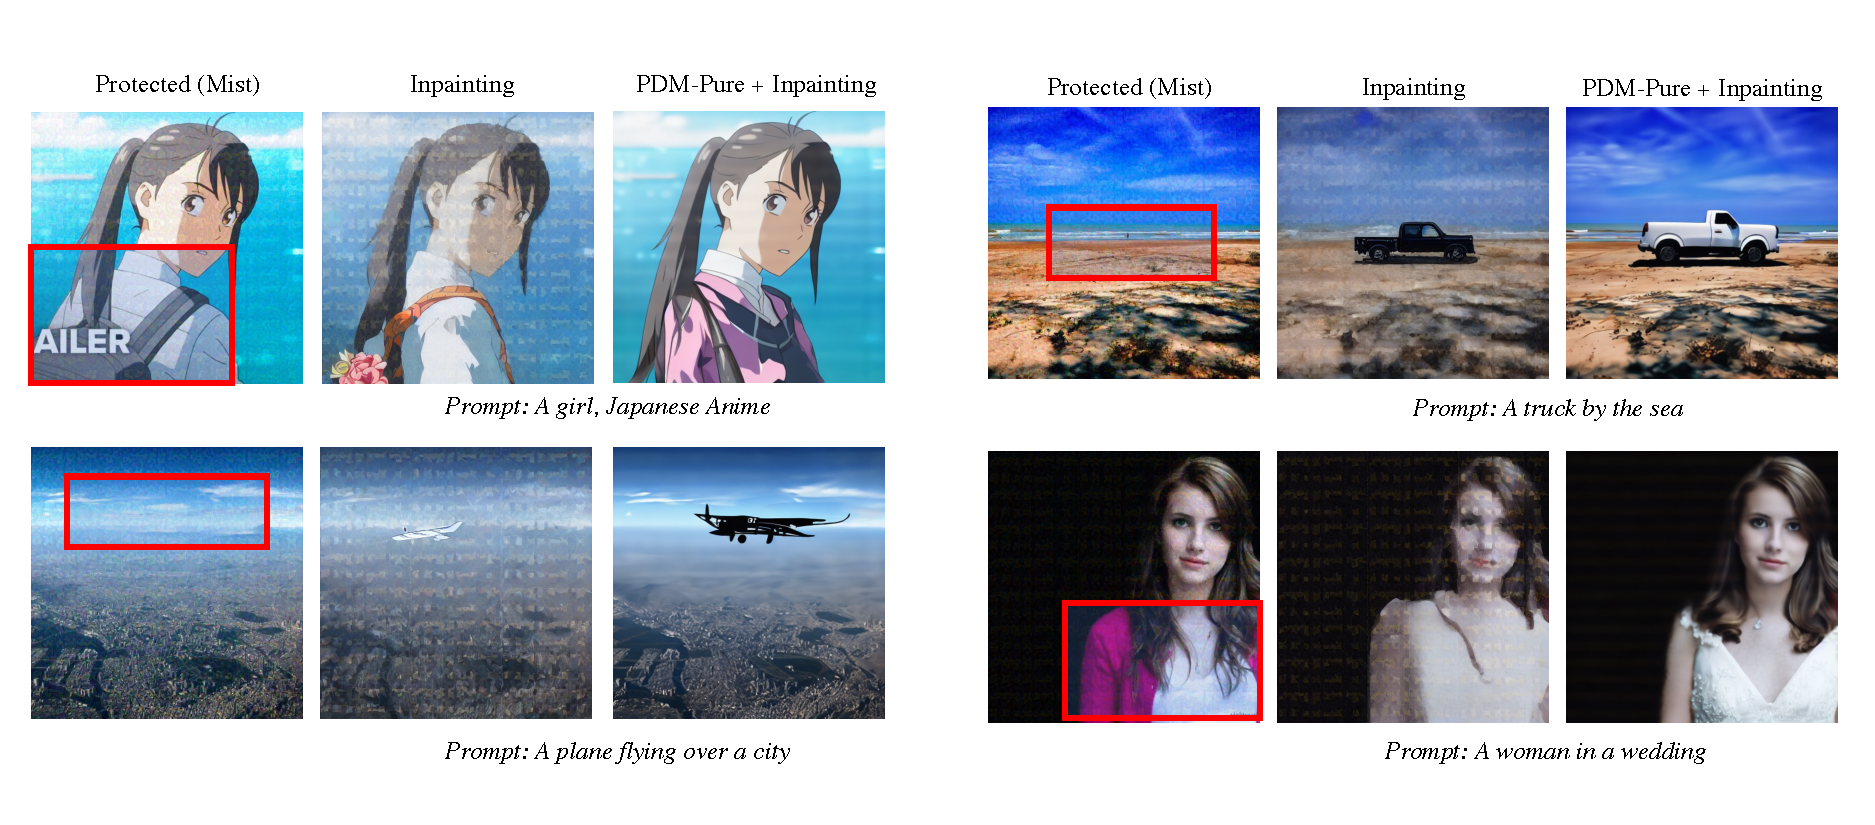
\includegraphics[width=.99\textwidth]{images/supp/pdm_pure_inpainting.pdf}
    \caption{\textbf{More Results of PDM-Pure Bypassing Protection for Inpainting}: after purification, the protected images can be easily inpainted with a high quality. The protective perturbations are generated using Mist with $\delta=16/255$, which is a strong perturbation.}
    \label{fig:supp:pdm_pure_inpainting}
\end{figure}




\begin{figure}
    \centering
    \includegraphics[width=.99\textwidth]{images/supp/pdm_pure_lora.pdf}
    \caption{\textbf{More Results of PDM-Pure Bypassing Protection for LoRA}: after purification, the protected images can be imitated again. Here we show examples using $5$ paintings of Claude Monet.}
    \label{fig:supp:pdm_pure_lora}
\end{figure}


\section{PDM-Pure For Higher Resolution}\label{supp:section:pdm_pure_for_higher_resolution}

In this paper, we mainly apply PDM-Pure for images sized $512\times 512$, which is also the most widely used resolution for latent diffusion models. When the resolution is $512\times 512$, running SDEdit using Stage II of DeepFloyd makes sense, while if the image size becomes larger, details may be lost because of the downsampling. Hopefully, we can still do purification patch-by-patch with PDM-Pure, in Figure~\ref{supp:section:pdm_pure_for_higher_resolution} we show purification results on images with different resolutions protected by Glaze~\cite{glaze}.


\begin{figure}
    \centering
    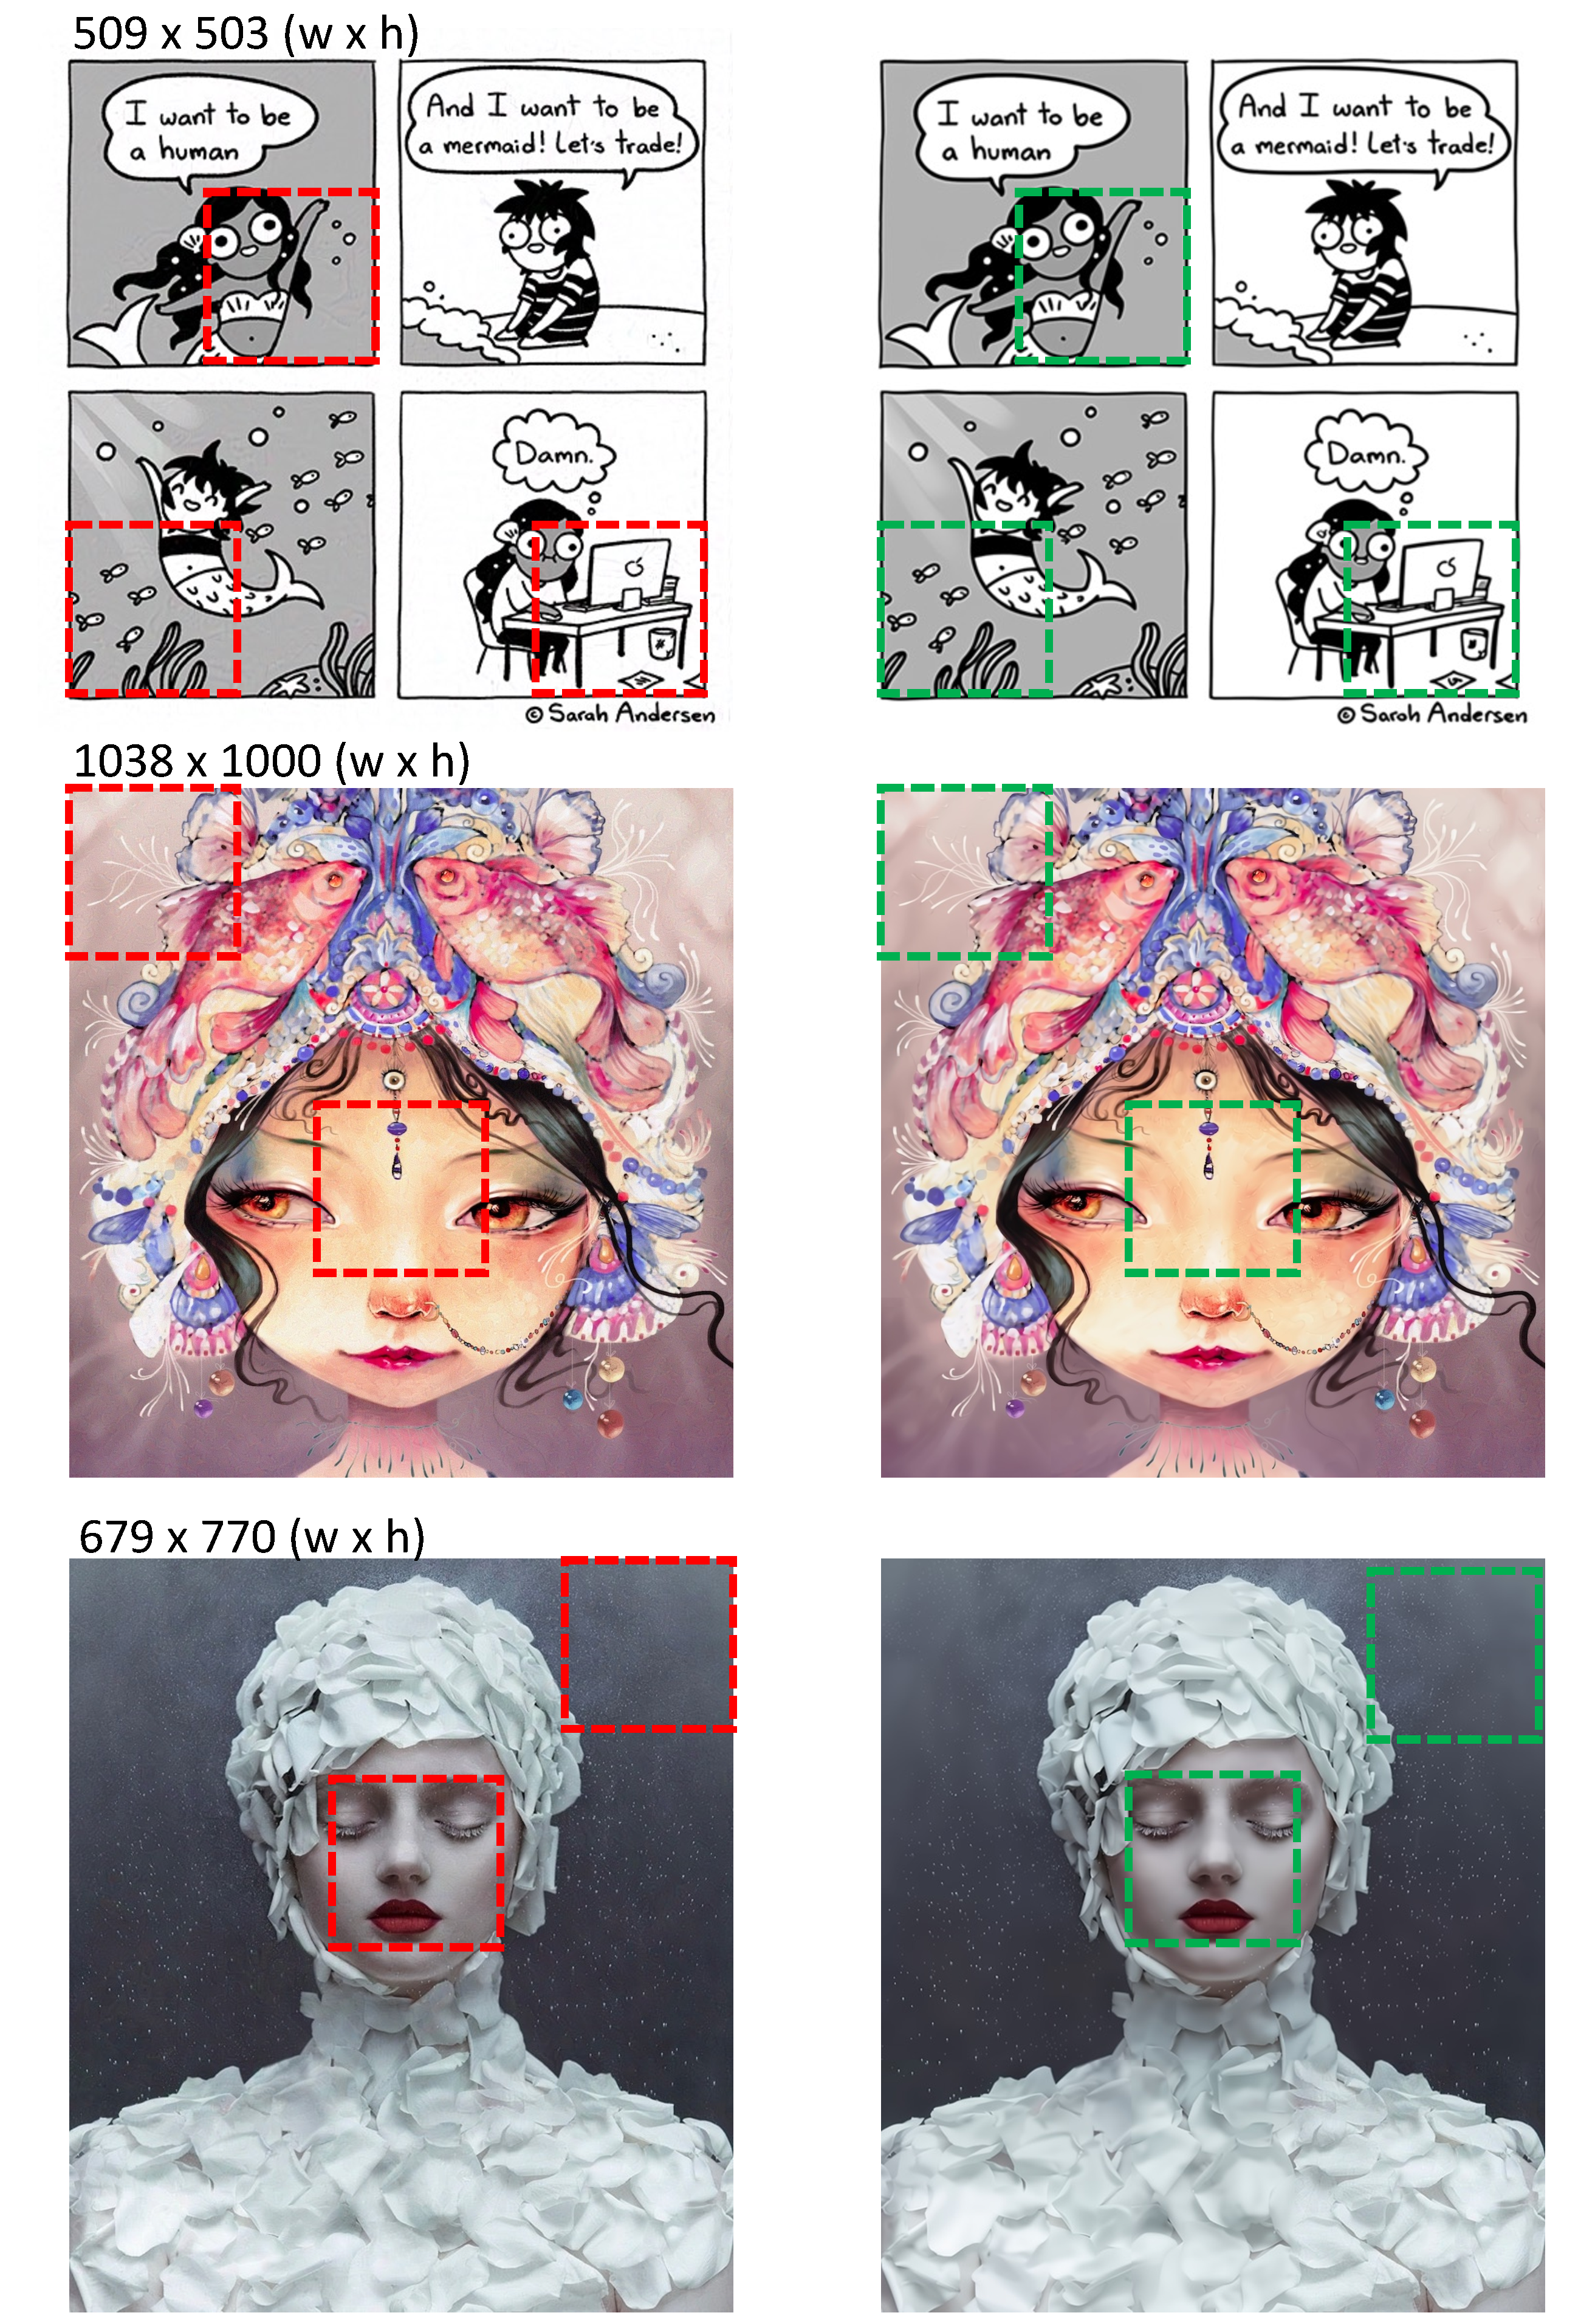
\includegraphics[width=.99\textwidth]{images/supp/larger_image_pdm_pure.pdf}
    \caption{\textbf{PDM-Pure Working On Images with Higher Resolution}: we show the results of applying PDM-Pure for images with higher resolutions, the images are protected using Glaze~\cite{glaze}. We can see from the figure that the adversarial patterns (in red box) can be effectively purified (in green box). Zoom in on the computer for a better view.}
    \label{fig:supp:pdm_pure_larger_image}
\end{figure}

\section{Ablations of $t^*$ in PDM-Pure}

The PDM-Pure on DeepFloyd-IF we used in this paper uses the default settings of SDEdit with $t^* = 0.1 T$. And we respace the diffusion model into $100$ steps, so we only need to run $10$ denoising steps. It can be run on one A6000 GPU, occupying $~22G$ VRAM in $30$ seconds.

Here we show some ablation about the choice of $t^*$. In fact, in many SDEdit papers, $t^*$ can be roughly defined by trying, different $t^*$ that can be used to purify different levels of noise. We try $t^*=0.01, 0.1, 0.2$, in Figure~\ref{fig:supp:pdm-pure_ablation} we can see that when $t^*=0.01$ the noise is not fully purified, and when $t^*=0.2$, the details in the painting are blurred. It should be noted that the sweet point for different images and different noises can be slightly different, so it will be more useful to do some trials before purification.



\begin{figure}
    \centering
    \includegraphics[width=.99\textwidth]{images/supp/pdm_pure_ablation.pdf}
    \caption{\textbf{PDM-Pure with Different $t^*$}}
    \label{fig:supp:pdm-pure_ablation}
\end{figure}




% \begin{table}[]
%     \centering
%     \begin{tabular}{cccccc}
%     \toprule
%         Model Name & Type & Structure & Resolution & Dataset & Resolution \\
%     \midrule
%       SD-V1.4~\cite{ldm}   & LDM & U-Net & 512 & LION & \\
%       SD-V1.5~\cite{ldm}  & LDM &U-Net & 512 & LION & \\
%       % SD-V2.1~\cite{ldm}  & LDM &U-Net & 512 & LION & \\
%       SD-XL~\cite{sdxl}  & LDM & U-Net & 512 & LION & \\
%       DeepFloyd Stage-I~\cite{deepfloyd} & PDM & U-Net & 64 & LION & \\
%       DeepFloyd Stage-II~\cite{deepfloyd} & PDM(c) & U-Net & 256 & LION & \\
%       Guided Diffusion a~\cite{guideddiffusion} & PDM & U-Net & 256 & ImageNet & \\
%       Guided Diffusion b~\cite{guideddiffusion}  & PDM & U-Net & 256 & LSUN-Bedroom & \\
%       Guided Diffusion c~\cite{guideddiffusion}  & PDM & U-Net& 256 & LSUN-Cat & \\
%       DiT-XL a~\cite{dit} & LDM & ViT & 256 & ImageNet & \\
%       DiT-XL b~\cite{dit}  & LDM & ViT & 512 & ImageNet & \\
%     \bottomrule
%     \end{tabular}
%     \caption{Models}
%     \label{tab:my_label}
% \end{table}

